%%%%%%%% ICML 2023 EXAMPLE LATEX SUBMISSION FILE %%%%%%%%%%%%%%%%%

\documentclass{article}

% Recommended, but optional, packages for figures and better typesetting:
\usepackage{microtype}
\usepackage{graphicx}
\usepackage{subfigure}
\usepackage{booktabs} % for professional tables

% hyperref makes hyperlinks in the resulting PDF.
% If your build breaks (sometimes temporarily if a hyperlink spans a page)
% please comment out the following usepackage line and replace
% \usepackage{icml2023} with \usepackage[nohyperref]{icml2023} above.
\usepackage[hyphens]{url}
\usepackage{hyperref}


% Attempt to make hyperref and algorithmic work together better:
\newcommand{\theHalgorithm}{\arabic{algorithm}}

% Use the following line for the initial blind version submitted for review:
%\usepackage{icml2023/icml2023}

% If accepted, instead use the following line for the camera-ready submission:
\usepackage[accepted]{icml2023/icml2023}

% For theorems and such
\usepackage{amsmath}
\usepackage{amssymb}
\usepackage{mathtools}
\usepackage{amsthm}

% if you use cleveref..
\usepackage[capitalize,noabbrev]{cleveref}

\usepackage{listings}

\lstset{basicstyle=\ttfamily\tiny}
\lstdefinestyle{mystyle}{
	keywordstyle=\bfseries,
	keywords={ge,return,def,not,xor,ne},
}
\lstset{breaklines=true}

%%%%%%%%%%%%%%%%%%%%%%%%%%%%%%%%
% THEOREMS
%%%%%%%%%%%%%%%%%%%%%%%%%%%%%%%%
\theoremstyle{plain}
\newtheorem{theorem}{Theorem}[section]
\newtheorem{proposition}[theorem]{Proposition}
\newtheorem{lemma}[theorem]{Lemma}
\newtheorem{corollary}[theorem]{Corollary}
\theoremstyle{definition}
\newtheorem{definition}[theorem]{Definition}
\newtheorem{assumption}[theorem]{Assumption}
\theoremstyle{remark}
\newtheorem{remark}[theorem]{Remark}

\makeatletter
\newcommand{\tleft}{\mathrel\triangleleft}
\newcommand{\tright}{\mathrel\triangleright}
\DeclareRobustCommand{\btleft}{\mathrel{\mathpalette\btlr@\blacktriangleleft}}
\DeclareRobustCommand{\btright}{\mathrel{\mathpalette\btlr@\blacktriangleright}}

\newcommand{\btlr@}[2]{%
	\begingroup
	\sbox\z@{$\m@th#1\triangleright$}%
	\sbox\tw@{\resizebox{1.1\wd\z@}{1.1\ht\z@}{\raisebox{\depth}{$\m@th#1\mkern-1mu#2$}}}%
	\ht\tw@=\ht\z@ \dp\tw@=\dp\z@ \wd\tw@=\wd\z@
	\copy\tw@
	\endgroup
}

\newcommand{\citemyauthoryear}[1]{\citeauthor{#1} (\citeyear{#1})}

% Todonotes is useful during development; simply uncomment the next line
%    and comment out the line below the next line to turn off comments
%\usepackage[disable,textsize=tiny]{todonotes}
\usepackage[textsize=tiny]{todonotes}

\usepackage{comment}

% The \icmltitle you define below is probably too long as a header.
% Therefore, a short form for the running title is supplied here:
\icmltitlerunning{Lossless hardening with $\partial\mathbb{B}$ nets}

\begin{document}

\twocolumn[
\icmltitle{Lossless hardening with $\partial\mathbb{B}$ nets}

% It is OKAY to include author information, even for blind
% submissions: the style file will automatically remove it for you
% unless you've provided the [accepted] option to the icml2023
% package.

% List of affiliations: The first argument should be a (short)
% identifier you will use later to specify author affiliations
% Academic affiliations should list Department, University, City, Region, Country
% Industry affiliations should list Company, City, Region, Country

% You can specify symbols, otherwise they are numbered in order.
% Ideally, you should not use this facility. Affiliations will be numbered
% in order of appearance and this is the preferred way.
\icmlsetsymbol{equal}{*}

\begin{icmlauthorlist}
\icmlauthor{Ian Wright}{comp}
\end{icmlauthorlist}

\icmlaffiliation{comp}{GitHub, Oxford, UK}

\icmlcorrespondingauthor{Ian Wright}{wrighti@acm.org}

% You may provide any keywords that you
% find helpful for describing your paper; these are used to populate
% the "keywords" metadata in the PDF but will not be shown in the document
\icmlkeywords{Machine Learning, ICML}

\vskip 0.3in
]

% this must go after the closing bracket ] following \twocolumn[ ...

% This command actually creates the footnote in the first column
% listing the affiliations and the copyright notice.
% The command takes one argument, which is text to display at the start of the footnote.
% The \icmlEqualContribution command is standard text for equal contribution.
% Remove it (just {}) if you do not need this facility.

%\printAffiliationsAndNotice{}  % leave blank if no need to mention equal contribution
\printAffiliationsAndNotice{{}} % otherwise use the standard text.

\begin{abstract}
		$\partial\mathbb{B}$ nets are differentiable neural networks that learn discrete boolean-valued functions by gradient descent. $\partial\mathbb{B}$ nets have two semantically equivalent aspects: a differentiable soft-net, with real weights, and a non-differentiable hard-net, with boolean weights. We train the soft-net by backpropagation and then `harden' the learned weights to yield boolean weights that bind with the hard-net. The result is a learned discrete function. Unlike existing approaches to neural network binarization the `hardening' operation involves no loss of accuracy. Preliminary experiments demonstrate that $\partial\mathbb{B}$ nets achieve comparable performance on standard machine learning problems yet are compact (due to 1-bit weights) and interpretable (due to the logical nature of the learnt functions).	
\end{abstract}

\vspace{-0.96cm}

\section{Introduction}

Neural networks must be differentiable. But differentiability means we cannot directly learn discrete functions, such as logical predicates. We can approximate discrete functions by defining continuous relaxations. This paper explores a different approach: we define differentiable functions that `harden', without approximation, to discrete functions. 

Specifically, $\partial \mathbb{B}$ nets have two aspects: a {\em soft-net}, which is a differentiable function with real weights, and a {\em hard-net}, which is a discrete function with boolean weights. Both aspects are semantically equivalent. We train the soft-net as normal, using backpropagation, then `harden' the learned weights to boolean values, which bind with the hard-net to yield a discrete function with identical predictive performance (see Figure \ref{fig:main-idea}).

\begin{figure}[h]
	\centering
	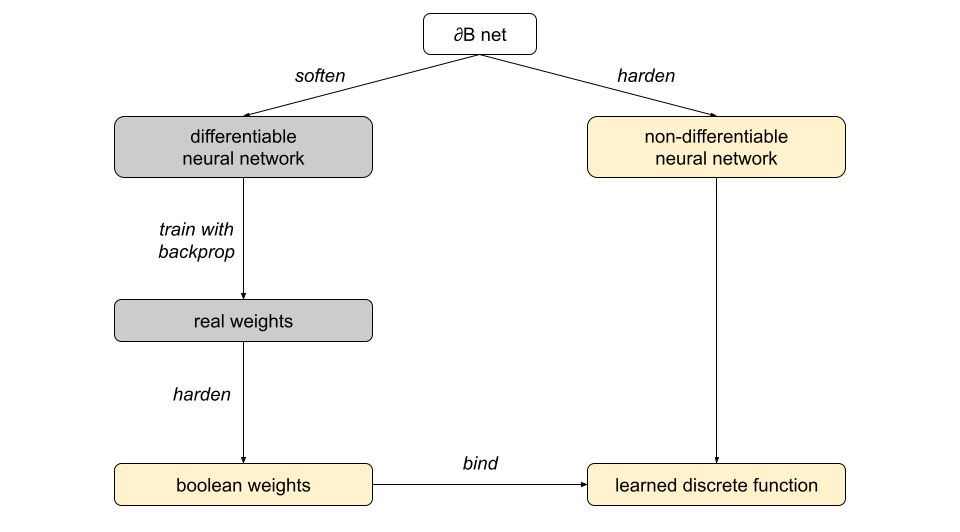
\includegraphics[trim=80pt 25pt 40pt 10pt, clip, width=0.5\textwidth]{../db-net.png}
	\caption{{\em Learning discrete functions with a $\partial\mathbb{B}$ net.}}
	\label{fig:main-idea}
\end{figure}

\section{$\partial\mathbb{B}$ nets}\label{sec:db-nets}

\begin{definition}[Soft-bits and hard-bits]
	A {\em soft-bit} is a real value in the range $[0,1]$ and a {\em hard-bit} is a boolean value from the set $\{0,1\}$. A soft-bit, $x$, is {\em high} if $x>1/2$, otherwise it is {\em low}.
\end{definition}
A hardening function converts soft-bits to hard-bits.
\begin{definition}[Hardening]
	The {\em hardening} function, $\operatorname{harden}(x_{1}, \dots, x_{n}) = [f(x_{1}), \dots, f(x_{n})]$, converts soft-bits to hard-bits, where $f(x)=1$ if $x > 1/2$ and $f(x)=0$ otherwise.
\end{definition}

Soft-nets use soft-bits and hard-nets use hard-bits. A soft-net learns 1-bit weights by representing them, at training time, as real numbers. The equivalent hard-net, at inference time, simply uses 1-bit weights. 
A soft-net is any differentiable, or differentiable a.e., function, $f$, that `hardens' to a hard-net that is a semantically equivalent discrete function, $g$.

\begin{definition}[Hard-equivalence]
	A function, $f: [0,1]^n \rightarrow [0,1]^m$, is {\em hard-equivalent} to a discrete function, $g: \{1,0\}^n \rightarrow \{1,0\}^m$,	if $\operatorname{harden}(f({\bf x})) = g(\operatorname{harden}({\bf x}))$
	for all ${\bf x} \in \{(x_{1}, \dots, x_{n}) ~|~ x_{i} \in [0,1] \setminus \{1/2\}\}$. For shorthand write $f \btright g$.
\end{definition}

$\partial \mathbb{B}$ nets are composed from `activation' functions that are hard-equivalent to boolean functions (and natural generalisations).

\subsection{Learning to negate}

Say we aim to learn to negate a boolean value, $x$, or leave it unaltered. Represent this decision by a boolean weight, $w$, where low $w$ means negate and high $w$ means do not. The boolean function that meets this requirement is $\neg(x \oplus w)$. However, this function is not differentiable. Define the differentiable function,
$\partial_{\neg}(w, x) = 1 - w + x (2w - 1)$,
where $\partial_{\neg}(w, x) \btright \neg(x \oplus w)$ (see proposition \ref{prop:not}).

Many kinds of differentiable fuzzy logic operators exist (see \citemyauthoryear{VANKRIEKEN2022103602} for a review). So why this functional form? Product logics, where $f(x,y) = x y$ is as a soft version of $x \wedge y$, although hard-equivalent at extreme values, e.g. $f(1,1)=1$ and $f(0,1)=0$, are not hard-equivalent at intermediate values, e.g. $f(0.6, 0.6) = 0.36$, which hardens to $\operatorname{False}$ not $\operatorname{True}$. G\"{o}del-style $\operatorname{min}$ and $\operatorname{max}$ functions, although hard-equivalent over the entire soft-bit range, i.e. $\operatorname{min}(x,y) \btright x \wedge y$ and $\operatorname{max}(x,y) \btright x \vee y$, are gradient-sparse in the sense that their outputs do not always vary when any input changes, e.g. $\frac{\partial}{\partial x} \operatorname{max}(x,y) = 0$ when $(x,y)=(0.1, 0.9)$. So although the composite function $\operatorname{max}(\operatorname{min}(w, x), \operatorname{min}(1-w, 1-x))$ is differentiable and $\btright \neg(x \oplus w)$ it does not always backpropagate error to its inputs. In contrast, $\partial_{\neg}$ always backpropagates error to its inputs because it is a gradient-rich function (see Figure \ref{fig:gradient-rich}). 

\begin{definition}[Gradient-rich]
	A function, $f: [0,1]^n \rightarrow [0,1]^m$, is {\em gradient-rich} if $\frac{\partial f({\bf x})}{\partial x_{i}} \neq {\bf 0}$ for all ${\bf x} \in \{(x_{1}, \dots, x_{n}) ~|~ x_{i} \in [0,1] \setminus \{1/2\}\}$.
\end{definition}

$\partial \mathbb{B}$ nets are composed of hard-equivalent `activation' functions that are, where possible, gradient-rich. To meet this requirement we introduce the technique of margin packing.

\subsection{Margin packing}

\begin{figure}[t!]
	\centering
	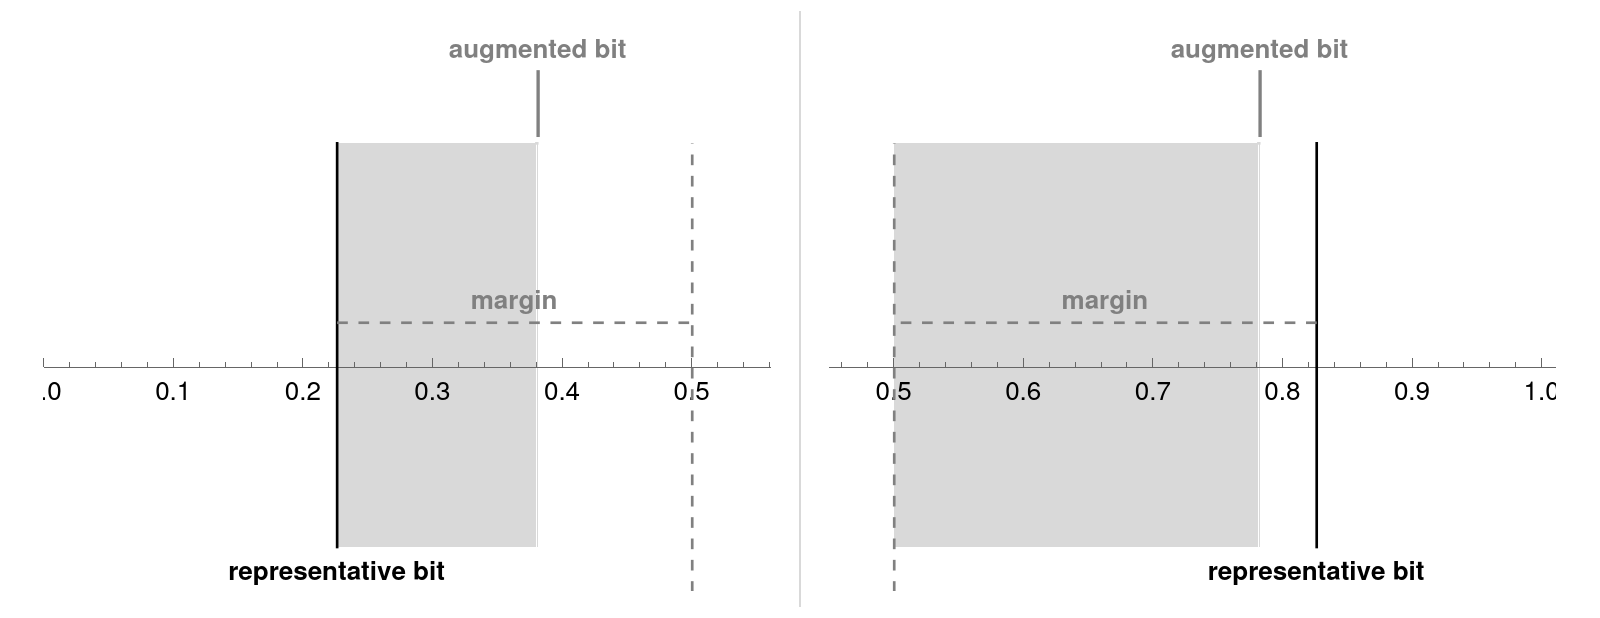
\includegraphics[trim=30pt 5pt 30pt 10pt, clip, width=.49\textwidth]{../margin-trick.png}
	\caption{{\em Margin packing for constructing gradient-rich, hard-equivalent functions}. A representative bit, $z$, is hard-equivalent to a discrete target function but gradient-sparse (e.g. $z=\operatorname{min}(x,y) \btright x \wedge y$). On the left $z$ is low, $z<1/2$; on the right $z$ is high, $z>1/2$. We can pack a fraction of the margin between $z$ and the hard threshold $1/2$ with additional gradient-rich information without affecting hard-equivalence. A natural choice is the mean soft-bit, $\bar{\bf x} \in [0,1]$. The grey shaded areas denote the packed margins and the final augmented bit. On the left $\approx 60\%$ of the margin is packed; on the right $\approx 90\%$.}
	\label{fig:margin-trick}
\end{figure}
% On the left, ${\bf x}=[0.9,0.23]$, $z=0.23$, $\bar{\bf x}=0.57$ and therefore $\approx 60\%$ of the margin is packed; on the right, ${\bf x}=[0.9,0.83]$,  $z=0.83$, $\bar{\bf x}=0.87$, and therefore $\approx 90\%$ of the margin is packed.

Say we aim to construct a differentiable analogue of $x \wedge y$. Note that $\operatorname{min}(x,y)$ essentially selects one of $x$ or $y$ as a representative soft-bit that is guaranteed hard-equivalent to $x \wedge y$. However, by selecting only one of $x$ or $y$ then $\operatorname{min}$ is also guaranteed to be gradient-sparse. We define a `margin packing' method to solve this dilemma.

The main idea of margin packing is (i) select a representative bit that is hard-equivalent to the target discrete function, and then (ii) pack a fraction of the margin between the representative bit and the hard threshold $1/2$ with gradient-rich information. The result is an augmented bit that is a function of all inputs yet hard-equivalent to the target function. More concretely, say a vector of soft-bit inputs ${\bf x}$ has an $i$th element that represents the target discrete function (e.g. if our target is $x \wedge y$ then ${\bf x}=[x,y]$ and $i$ is 1 if $x<y$ and $i=2$ otherwise). Now, if we pack only a fraction of the available margin, $|x_{i}-1/2|$, we will not cross the $1/2$ threshold and break the hard-equivalence of the representative bit. The average soft-bit value, $\bar{\bf x} \in [0,1]$, is just such a gradient-rich fraction. We therefore define $\operatorname{margin-fraction}({\bf x}, i) = \bar{\bf x} \times \left|x_{i} - 1/2\right|$. The packed fraction, $\bar{\bf x}$, of the margin increases or decreases with the average soft-bit value. The available margin, $\left|x_{i} - 1/2\right|$, tends to zero as the representative bit, $x_{i}$, tends to the hard threshold $1/2$. At the threshold point there is no margin to pack. Now, define the augmented bit as
\begin{equation}
\begin{aligned}
&\operatorname{augmented-bit}({\bf x}, i) =\\
& ~~~~~~ 
\begin{cases}
1/2 + \operatorname{margin-fraction}({\bf x}, i) & \text{if } x_{i} > 1/2 \\
x_{i} + \operatorname{margin-fraction}({\bf x}, i) & \text{otherwise,}
\end{cases}
\end{aligned}
\label{eq:augmented-bit}
\end{equation}
which is differentiable a.e. Note that if the representative bit is high (resp. low) then the augmented bit is also high (resp. low). The difference between the augmented and representative bit depends on the size of the available margin and the mean soft-bit value. Almost everywhere, an increase (resp. decrease) of the mean soft-bit increases (resp. decreases) the value of the augmented bit (see Figure \ref{fig:margin-trick}). Note that if the $i$th bit is representative (i.e. hard-equivalent to the target function) then so is the augmented bit (see lemma \ref{prop:augmented}). We use margin packing, where appropriate, to define gradient-rich, hard-equivalents of boolean functions.

\subsection{Differentiable $\wedge$, $\vee$ and $\Rightarrow$}

\begin{figure*}[t!]
	\centering
	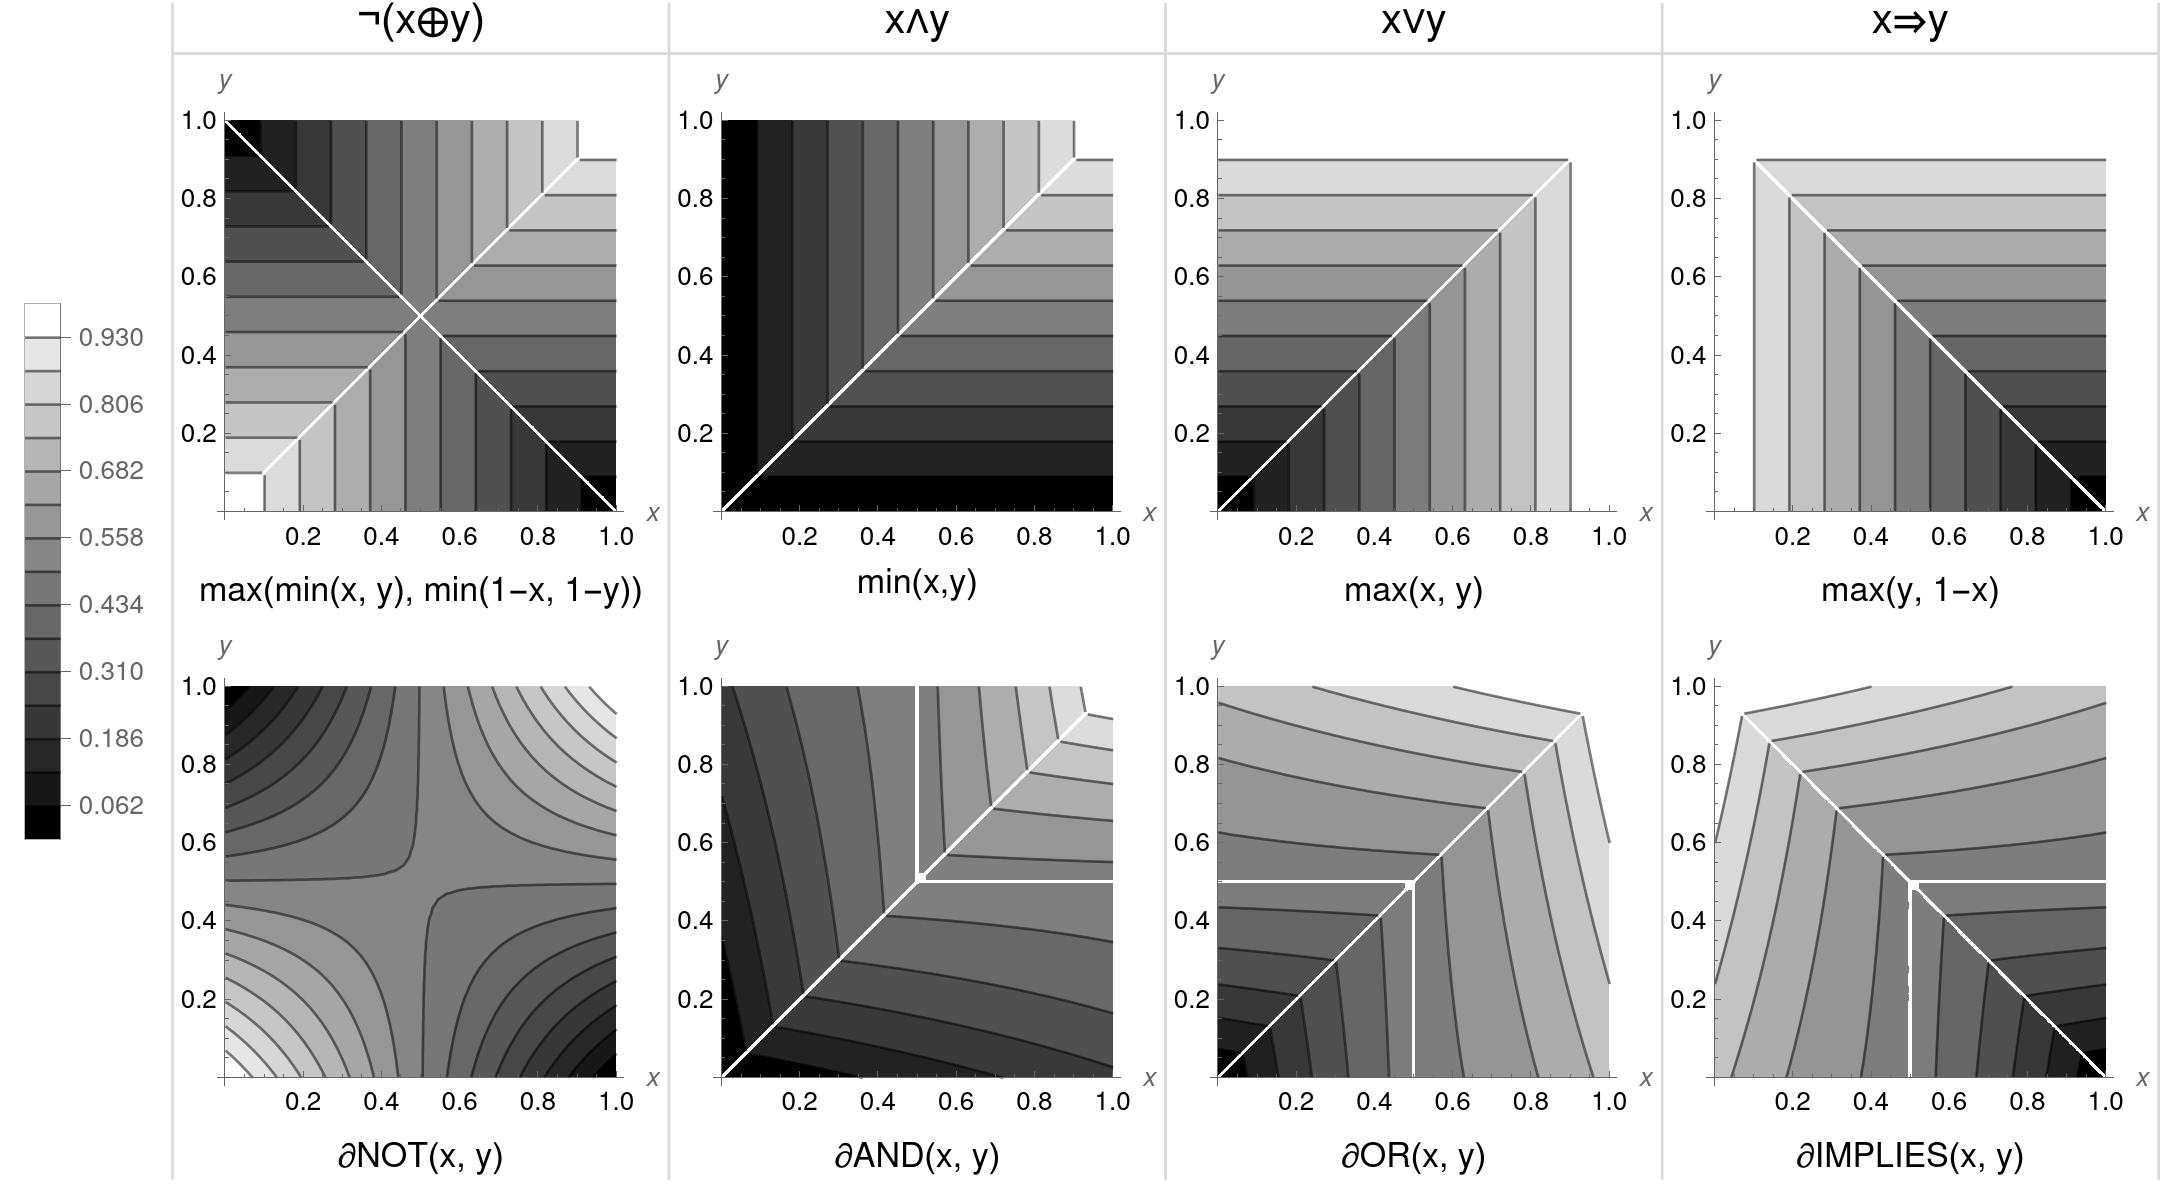
\includegraphics[trim=0pt 0pt 0pt 0pt, clip, width=0.8\textwidth]{../logic-gates.png}
	\caption{{\em Gradient-rich versus gradient-sparse differentiable boolean functions.} Each column contains contour plots of functions $f(x,y)$ that are hard-equivalent to a boolean function (one of $\neg(x \oplus y)$, $x \wedge y$, $x \vee y$, or $x \Rightarrow y$). Every function is continuous and differentiable a.e. (white lines indicate non-continuous derivatives). The upper plots are gradient-sparse, where vertical and horizontal contours indicate the function is constant with respect to one of its inputs, i.e. $\partial f/\partial y = 0$ or $\partial f/\partial x = 0$. The lower plots are gradient-rich, where the curved contours indicate the function always varies with respect to any of its inputs, i.e. $\partial f/\partial y \neq 0$ and $\partial f/\partial x \neq 0$. $\partial \mathbb{B}$ nets use gradient-rich functions to ensure that error is always backpropagated to all inputs.} 
	\label{fig:gradient-rich}
\end{figure*}

We aim to construct a differentiable analogue of the boolean function $\bigwedge_{i=1}^{n} x_i$. A representative bit is $\operatorname{min}(x_{1},\dots,x_{n})$. The function
$\partial_{\wedge}({\bf x}) = \operatorname{augmented-bit}({\bf x}, \operatorname{argmin}\limits_{i} x[i])$
is therefore hard-equivalent to the boolean function $\bigwedge_{i=1}^{n} x_i$ (see proposition \ref{prop:and}). In the special case $n=2$ we get the piecewise function,
$\partial_{\wedge}\!(x, y) = 1/2 + 1/2(x + y)(\operatorname{min}(x,y) - 1/2)$ if $\operatorname{min}(x,y) > 1/2$, and $\partial_{\wedge}\!(x, y) = \operatorname{min}(x,y) + 1/2(x + y)(1/2 - \operatorname{min}(x,y))$
otherwise. Note that $\partial_{\wedge}$ is differentiable a.e. and gradient-rich (see Figure \ref{fig:gradient-rich}). The differentiable analogue of $\vee$ is identical to $\wedge$, except the representative bit is selected by $\operatorname{max}$. The function
$\partial_{\vee}({\bf x}) = \operatorname{augmented-bit}({\bf x}, \operatorname{argmax}\limits_{i} x[i])$ is hard-equivalent to the boolean function $\bigvee_{i=1}^{n} x_i$ (see proposition \ref{prop:or}) (see Figure \ref{fig:gradient-rich}).
The differentiable analogue of $\Rightarrow$ (material implication) is defined in terms of $\partial_{\vee}$. The function
$\partial_{\Rightarrow}(x, y) = \partial_{\vee}\!(y, 1-x)$,
is hard-equivalent to $x \Rightarrow y$ (see proposition \ref{prop:implies}). We can define  analogues of all the basic boolean operators in a similar manner.

\subsection{Differentiable majority}

\begin{figure*}[t]
	\centering
	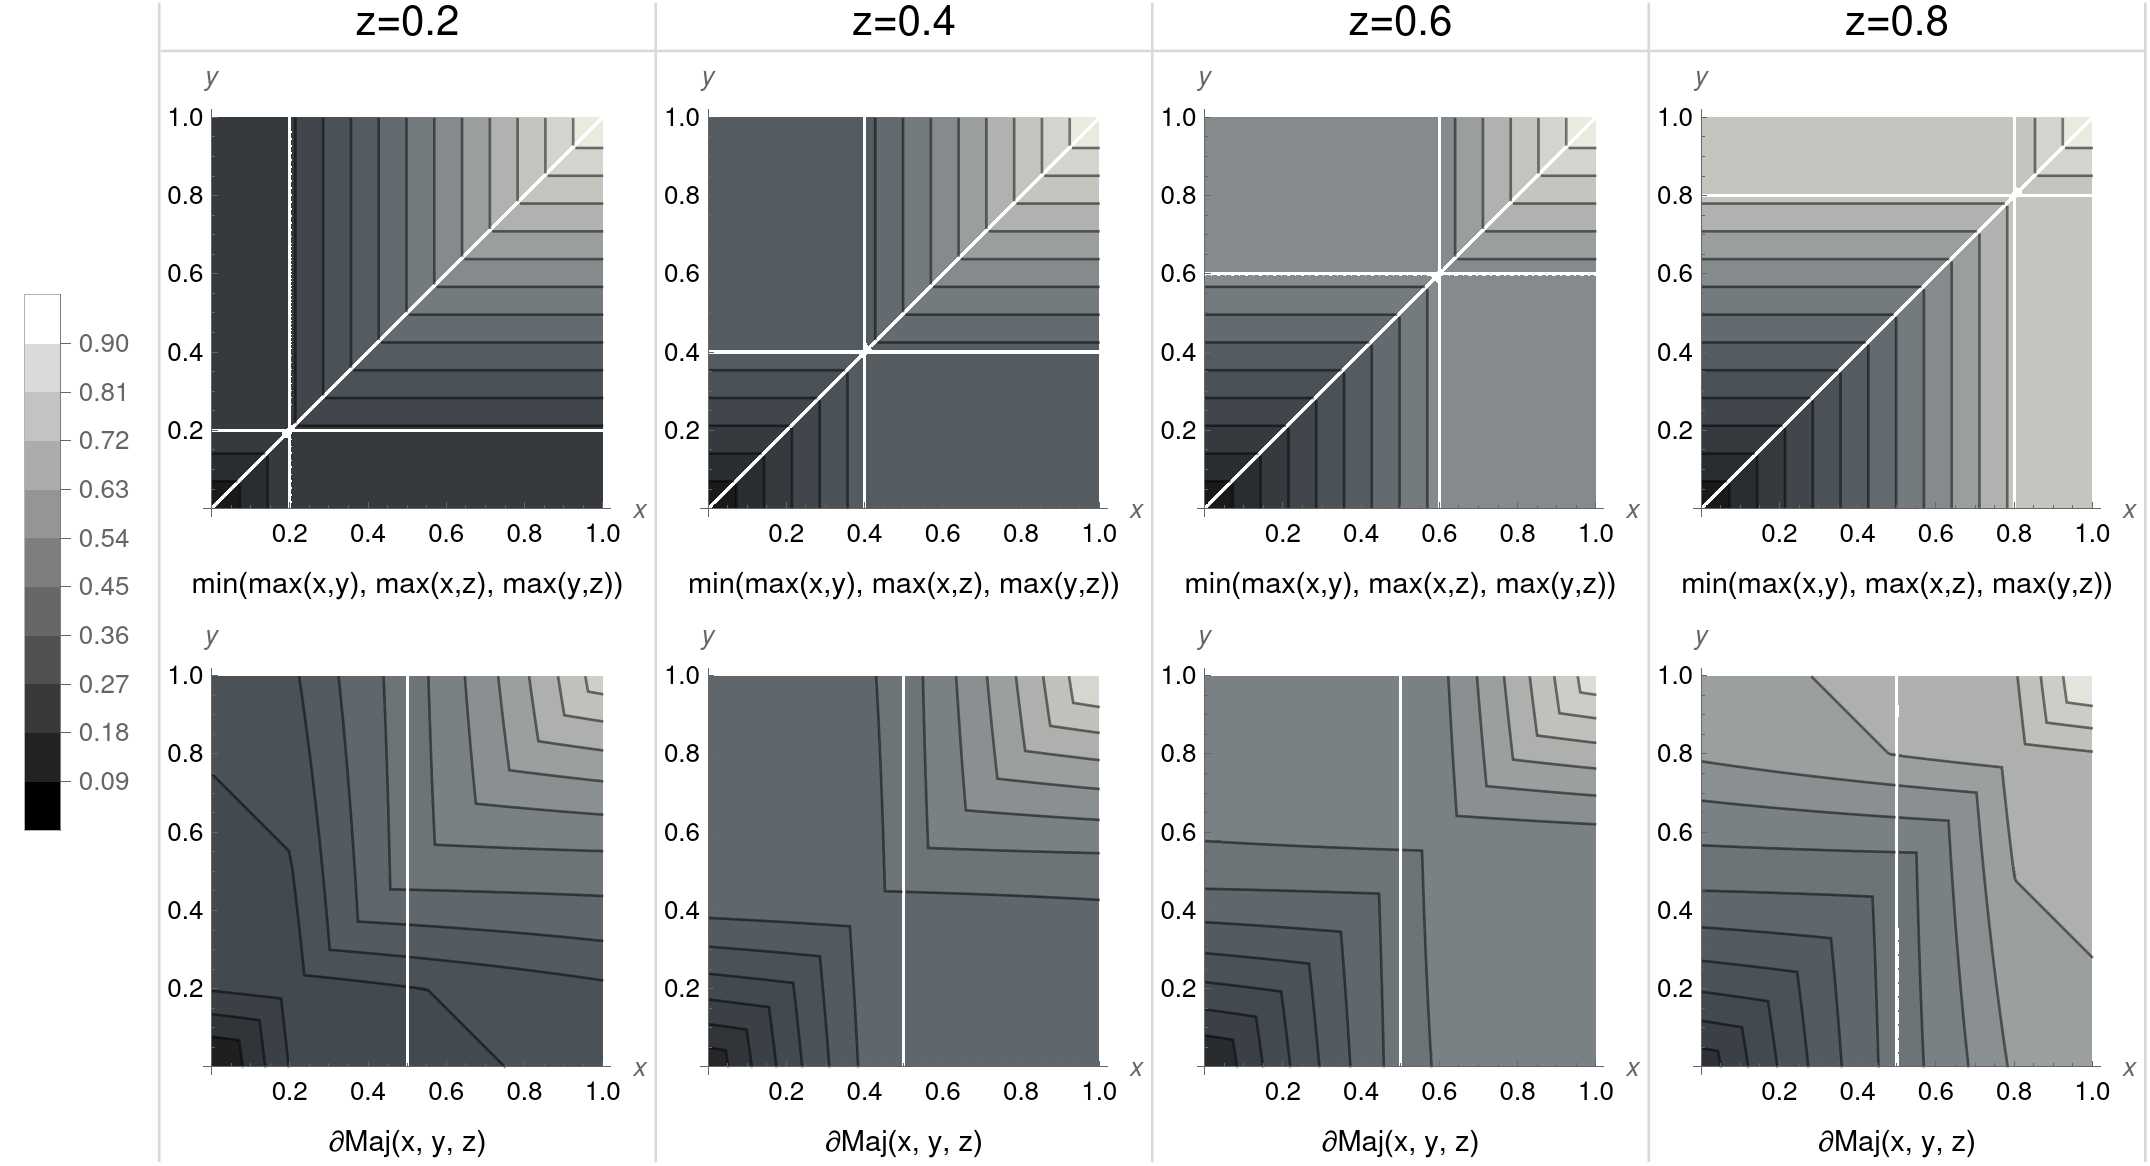
\includegraphics[trim=0pt 0pt 0pt 0pt, clip, width=0.8\textwidth]{../majority-gates.png}
	\caption{{\em Differentiable boolean majority.} The boolean majority function for three variables in DNF form is $\operatorname{Maj}(x,y,z) = (x \wedge y) \vee (x \wedge y) \vee (y \wedge z)$. The upper row contains contour plots of $f(x,y,z) = \operatorname{min}(\operatorname{max}(x,y), \operatorname{max}(x,z), \operatorname{max}(y,z))$ for values of $z \in \{0.2, 0.4, 0.6, 0.8\}$. $f$ is differentiable and $\btright\!\operatorname{Maj}$ but gradient-sparse (vertical and horizontal contours indicate constancy with respect to an input). Also, the number of terms in $f$ grows exponentially with the number of variables. The lower row contains contour plots of $\partial\!\operatorname{Maj}(x,y,z)$ for the same values of $z$. $\partial\!\operatorname{Maj}$ is differentiable and $\btright\!\operatorname{Maj}$ yet gradient-rich (curved contours indicate variability with respect to any inputs). In addition, the number of terms in $\partial\!\operatorname{Maj}$ is constant with respect to the number of variables.} 
	\label{fig:majority-plot}
\end{figure*}

The boolean majority function is particularly important for tractable learning because it is a threshold function:
\begin{equation*}
\begin{aligned}
\operatorname{Maj}({\bf x}) &= \left\lfloor
\frac{1}{2} + \frac{\sum_{i=1}^{n} x_{i} - 1/2}{n}
\right\rfloor\text{,}
\end{aligned}
\end{equation*}
where we count $\operatorname{False}$ as $0$ and $\operatorname{True}$ as $1$. We aim to construct a differentiable analogue of $\operatorname{Maj}$.

$\operatorname{Maj}$ for $n$ bits in DNF form is a disjunction of $\binom{n}{k}$ conjunctive clauses of size $k$, where $k=\lceil n/2 \rceil$. In principle we can implement a differentiable analogue of $\operatorname{Maj}$ in terms of $\partial_{\wedge}$ and $\partial_{\vee}$. However, the number of terms grows exponentially with the variables. No general algorithm exists to find the minimal representation of $\operatorname{Maj}$ for arbitrary $n$. Instead, we trade-off time for memory costs. Assume that the function $\operatorname{sort}({\bf x})$ sorts the elements of ${\bf x}$ in ascending order. Then the `median' soft-bit,
$\operatorname{majority-index}({\bf x}) = \lceil \frac{|{\bf x}|}{2} \rceil$,
is representative. Applying margin packing, define the differentiable function
$\partial\!\operatorname{Maj}({\bf x}) = \operatorname{augmented-bit}(\operatorname{sort}({\bf x}), \operatorname{majority-index}({\bf x}))$,
which is hard-equivalent to $\operatorname{Maj}$ (see theorem \ref{prop:majority}). Note that $\partial\!\operatorname{Maj}$ is differentiable a.e. and gradient-rich (see Figure \ref{fig:majority-plot}). If $\operatorname{sort}$ is quicksort then the average time-complexity of $\partial\!\operatorname{Maj}$ is $\mathcal{O}(n\log{}n)$, which makes $\partial\!\operatorname{Maj}$ more expensive than $\partial_{\neg}$, $\partial_{\wedge}$, $\partial_{\vee}$ and $\partial_{\Rightarrow}$ at training time. The $\operatorname{sort}$ operation could be replaced by the Floyd-Rivest algorithm, which has linear average time complexity \cite{KIWIEL2005214}. However, in the hard $\partial\mathbb{B}$ net we efficiently implement $\operatorname{Maj}$ as a discrete program that simply checks if the majority of bits are high. Note that we use $\operatorname{sort}$ to define a differentiable function that is exactly equivalent to a discrete function (rather than defining a continuous approximation to sorting, e.g. \citemyauthoryear{NEURIPS2019_d8c24ca8}, \citemyauthoryear{grover2018stochastic} and \citemyauthoryear{petersen2022monotonic}).

We apply this methodology to construct functions that harden to other kinds of boolean functions, such as boolean counting (see Section \ref{sec:counting}). This basic set of functions is sufficient to learn non-trivial relationships from data. $\partial\mathbb{B}$ net layers are compositions of these functions, where composition preserves hard-equivalence  (see Sections \ref{sec:layers} and \ref{sec:classification}). 

\section{Learning discrete functions}\label{sec:discrete}

We briefly illustrate the kind of discrete program that $\partial\mathbb{B}$ nets can learn. Consider the toy problem of predicting whether a person wears a $\operatorname{t-shirt}$ (label 0) or a $\operatorname{coat}$ (label 1) conditional on 5 boolean features (see Table \ref{tab:toy2}).

\begin{table}[h!]
	\centering
	\begin{tabular}{|c|c|c|c|c|c|}
		$\text{\small very-cold}$ & $\text{\small cold}$ & $\text{\small warm}$ & $\text{\small very-warm}$ & $\text{\small outside}$ & $\text{\small label}$ \\ \hline
		1 & 0 & 0 & 0 & 0 & 1 \\
		0 & 0 & 0 & 1 & 1 & 1 \\
		0 & 0 & 1 & 0 & 1 & 0 \\
		0 & 0 & 0 & 1 & 0 & 0 \\
		\dots & \dots & \dots & \dots & \dots & \dots
	\end{tabular}
	\caption{A toy learning problem}
	\label{tab:toy2}
\end{table}

We train the $\partial\mathbb{B}$ net described in Figure 5\ref{fig:toy-example-architecture}. Once trained we harden the net to a discrete program (see Section \ref{sec:discrete}) that generates 2 hard-bits, corresponding to each label. The program symbolically simplifies to:

\begin{lstlisting}[language=Python,style=mystyle,frame=single]
def dbNet(very-cold, cold, warm, very-warm, outside):
return [
4 !very-cold + 4 !cold + (3 warm + !warm) + (very-warm + 3 !very-warm) + (outside + 3 !outside) >= 11,
(very-cold + 3 !very-cold) + 4 cold + 4 !warm + (3 very-warm + !very-warm) + 2 (outside + !outside) >= 11
]
\end{lstlisting}

Note that the program linearly weights multiple pieces of evidence due to the presence of the $\partial\!\operatorname{Maj}$ operator (overkill for this toy problem). We can read-off that the $\partial\mathbb{B}$ net has learned `if not $\operatorname{very-cold}$ and not $\operatorname{cold}$ and not $\operatorname{outside}$ then wear a $\operatorname{t-shirt}$'; and `if $\operatorname{cold}$ and not ($\operatorname{warm}$ or $\operatorname{very-warm}$) and $\operatorname{outside}$ then wear a $\operatorname{coat}$' etc. Section \ref{sec:experiments} compares $\partial\mathbb{B}$ net performance against other classification algorithms on standard machine learning problems.

\section{Related work}

Binary neural networks, e.g. \citemyauthoryear{10.5555/2969442.2969588}, reduce real weights and/or activations to binary, saving model size and inference costs. The binarization step is lossy, which loses accuracy \citep{QIN2020107281}. Deep differentiable logic gate networks \citep{NEURIPS2022_0d3496dd} consist of 2-input neurons arranged in a fixed topology. Each neuron learns a differentiable probability distribution over the 16 possible binary functions. Post-training the neurons are discretized to the most probable binary function. This step is lossy, which loses accuracy. $\partial\mathbb{B}$ nets aim to explore the design space of differentiable nets that enable lossless hardening.

\section{Conclusion}\label{sec:conclusion}

$\partial\mathbb{B}$ nets are differentiable nets that are hard-equivalent to non-differentiable, boolean-valued functions. $\partial\mathbb{B}$ nets can therefore learn discrete functions by gradient descent. Ensuring hard-equivalence requires defining new kinds of activation functions and network layers. `Margin packing' is a potentially general technique for constructing differentiable functions that are hard-equivalent yet gradient-rich. An advantage of $\partial\mathbb{B}$ nets is that `hardening' to 1-bit weights has provably identical accuracy. At inference time $\partial\mathbb{B}$ nets are highly compact and potentially cheap to evaluate. Preliminary experiments demonstrate that $\partial\mathbb{B}$ nets achieve comparable performance to existing approaches. 

% Acknowledgements should only appear in the accepted version.
\section*{Acknowledgements}
GitHub Next sponsored this research. Thanks to Pavel Augustinov, Richard Evans, Johan Rosenkilde, Max Schaefer, Ganesh Sittampalam, Tam\'{a}s Szab\'{o}, Albert Ziegler and the anonymous referees for helpful discussions and feedback.

\bibliography{../db.bib}
\bibliographystyle{icml2023/icml2023}


%%%%%%%%%%%%%%%%%%%%%%%%%%%%%%%%%%%%%%%%%%%%%%%%%%%%%%%%%%%%%%%%%%%%%%%%%%%%%%%
%%%%%%%%%%%%%%%%%%%%%%%%%%%%%%%%%%%%%%%%%%%%%%%%%%%%%%%%%%%%%%%%%%%%%%%%%%%%%%%
% APPENDIX
%%%%%%%%%%%%%%%%%%%%%%%%%%%%%%%%%%%%%%%%%%%%%%%%%%%%%%%%%%%%%%%%%%%%%%%%%%%%%%%
%%%%%%%%%%%%%%%%%%%%%%%%%%%%%%%%%%%%%%%%%%%%%%%%%%%%%%%%%%%%%%%%%%%%%%%%%%%%%%%
\newpage
\appendix
\onecolumn

\section{Boolean logic layers}\label{sec:layers}

The full variety of $\partial\mathbb{B}$ net architectures is to be explored. Here we define basic layers sufficient for the classification experiments.

A $\partial_{\neg} \!\operatorname{Layer}$ of width $n$ learns to negate up to $n$ different subsets of the elements of its input vector:
\begin{equation*}
\begin{aligned}
& \partial_{\neg} \!\operatorname{Layer}: [0,1]^{n \times m} \times [0,1]^{m} \to [0,1]^{n \times m}, \\
({\bf W}, {\bf x}) &\mapsto 
\begin{bmatrix}
\partial_{\neg}(w_{1,1}, x_{1}) & \dots & \partial_{\neg}(w_{1,m}, x_{m}) \\
\vdots & \ddots & \vdots \\
\partial_{\neg}(w_{n,1}, x_{1}) & \dots & \partial_{\neg}(w_{n,m}, x_{m})
\end{bmatrix}
\end{aligned}
\end{equation*}
where ${\bf x}$ is a soft-bit input vector, ${\bf W}$ is a weight matrix and $n$ is the layer width. Similarly, A $\partial_{\Rightarrow} \!\operatorname{Layer}$ of width $n$ learns to `mask to true or $\operatorname{nop}$' up to $n$ different subsets of the elements of its input vector:
\begin{equation*}
\partial_{\Rightarrow} \!\operatorname{Layer}({\bf W}, {\bf x}) =
\begin{bmatrix}
\partial_{\Rightarrow}(w_{1,1}, x_{1}) & \dots & \partial_{\Rightarrow}(w_{1,m}, x_{m}) \\
\vdots & \ddots & \vdots \\
\partial_{\Rightarrow}(w_{n,1}, x_{1}) & \dots & \partial_{\Rightarrow}(w_{n,m}, x_{m})
\end{bmatrix}\text{.}
\end{equation*}
A $\partial_{\wedge}\!\operatorname{Neuron}$ learns to logically $\wedge$ a subset of its input vector:
\begin{equation*}
\begin{aligned}
& \partial_{\wedge}\!\operatorname{Neuron}: [0,1]^{n} \times [0,1]^{n} \to [0,1], \\
({\bf w}, {\bf x}) & \mapsto \min(\partial_{\Rightarrow}\!(w_{1}, x_{1}), \dots, \partial_{\Rightarrow}\!(w_{n}, x_{n}))\text{,}
\end{aligned}
\end{equation*}
where ${\bf w}$ is a weight vector. Each $\partial_{\Rightarrow}(w_{i},x_{i})$ learns to include or exclude $x_{i}$ from the conjunction depending on weight $w_{i}$. For example, if $w_{i}>0.5$ then $x_{i}$ affects the value of the conjunction since $\partial_{\Rightarrow}(w_{i},x_{i})$ passes-through a soft-bit that is high if $x_{i}$ is high, and low otherwise; but if $w_{i} \leq 0.5$ then $x_{i}$ does not affect the conjunction since $\partial_{\Rightarrow}(w_{i},x_{i})$ always passes-through a high soft-bit. A $\partial_{\wedge}\!\operatorname{Layer}$ of width $n$ learns up to $n$ different conjunctions of subsets of its input (of whatever size). A $\partial_{\vee}\!\operatorname{Neuron}$ is defined similarly:
\begin{equation*}
\begin{aligned}
& \partial_{\vee}\!\operatorname{Neuron}: [0,1]^{n} \times [0,1]^{n} \to [0,1], \\
({\bf w}, {\bf x}) &\mapsto \max(\partial_{\wedge}\!(w_{1}, x_{1}), \dots, \partial_{\wedge}\!(w_{n}, x_{n}))\text{.}
\end{aligned}
\end{equation*}
Each $\partial_{\wedge}(w_{i},x_{i})$ learns to include or exclude $x_{i}$ from the disjunction depending on weight $w_{i}$. A $\partial_{\vee}\!\operatorname{Layer}$ of width $n$ learns up to $n$ different disjunctions of subsets of its input (of whatever size).
%For example, if $w_{i}>0.5$ then $x_{i}$ affects the value of the conjunction because $\partial_{\wedge}(w_{i},x_{i})$ passes-through a soft-bit that is high if $x_{i}$ is high, and low otherwise; but if $w_{i} \leq 0.5$ then $x_{i}$ does not affect the conjunction because $\partial_{\Rightarrow}(w_{i},x_{i})$ always passes-through a low soft-bit. 

We can compose $\partial_{\neg}$, $\partial_{\wedge}$ and $\partial_{\vee}$ layers to learn boolean formulae of arbitrary width and depth.

\section{Classification layers}\label{sec:classification}

In classification problems the final layer of a neural network is typically interpreted as a vector of real-valued logits, one for each label, where the index of the maximum logit indicates the most probable label. However, we cannot interpret a soft-bit vector as logits without violating hard-equivalence. In addition, when training $\partial\mathbb{B}$ nets, loss functions should be a function of hardened bits, otherwise gradient descent may non-optimally traverse trajectories that take no account of the hard threshold at $1/2$. For example, consider that an instance is correctly classified by a 1-hot vector with high bit $x=0.51$. Updating the net's weights to change this value to $0.51+\epsilon$ will not improve accuracy and may prevent the correct classification of a different instance. 

For these reasons, $\partial\mathbb{B}$ nets have a final `hardening' layer to ensure that loss is a function of hard, not soft, bits:
\begin{equation*}
\begin{aligned}
\partial\!\operatorname{harden}: [0,1]^{n} &\to [0,1]^{n}, \\
{\bf x} &\mapsto \operatorname{harden}({\bf x})\text{.}
\end{aligned}
\end{equation*}
The $\operatorname{harden}$ function is not differentiable and therefore $\partial\!\operatorname{harden}$ uses the straight-through estimator \cite{DBLP:journals/corr/BengioLC13} during backpropagation. By restricting the use of the straight-through estimator to final layers we avoid compounding gradient estimation errors to deeper parts of the network. Note that $\partial\!\operatorname{harden}$ is hard-equivalent to a $\operatorname{nop}$.

$\partial\mathbb{B}$ nets can re-use many of the techniques deployed in standard neural networks. For example, for improved generalisation, we define a `boolean' analogue of the dropout layer \cite{JMLR:v15:srivastava14a}:
\begin{equation*}
\begin{aligned}
\partial\!\operatorname{dropout}: [0,1]^{n} \times [0,1] &\to [0,1]^{n}, \\
({\bf x}, p) &\mapsto [f(x_{1}, p), \dots, f(x_{n}, p)]\text{,}
\end{aligned}
\end{equation*}
where
\begin{equation*}
f(x, p) = \begin{cases}
1 - x, & \text{with probability } p \\
x, & \text{otherwise.}
\end{cases}
\end{equation*}
At train time $\partial\!\operatorname{dropout}$ randomly negates soft-bit values with probability $p$. At test time, and in the hard-net, $\partial\!\operatorname{dropout}$ is a $\operatorname{nop}$.

\section{Differentiable counting}\label{sec:counting}

A boolean counting function $f({\bf x})$ is $\operatorname{True}$ if a counting predicate, $c({\bf x})$, holds over its $n$ inputs. We aim to construct a differentiable analogue of $\operatorname{count}({\bf x}, k)$ where $c({\bf x}) := |\{x_{i} : x_{i} = 1 \}| = k$ (i.e. `exactly $k$ high'), which can be useful in multiclass classification problems. Define
\begin{equation*}
\begin{aligned}
\partial\!\operatorname{count-hot}: [0,1]^{n} &\to [0,1]^{n+1}, \\
{\bf x} &\mapsto \operatorname{low-high}(\operatorname{sort}({\bf x}))\text{,}
\end{aligned}
\end{equation*}
where 
\begin{equation*}
\begin{aligned}
& \operatorname{low-high}: [0,1]^{n} \to [0,1]^{n+1},\\
& {\bf x} \mapsto \left[ \partial_{\wedge}\!(1, x_{1}), \partial_{\wedge}\!(1 - x_{1}, x_{2}), \dots, 
\partial_{\wedge}\!(1 - x_{n-1}, x_{n}), \partial_{\wedge}\!(1-x_{n}, 1) \right]\text{.}
\end{aligned}
\end{equation*}
$\partial\!\operatorname{count-hot}({\bf x})$ outputs a 1-hot vector where the index of the high bit is the number of low bits in ${\bf x}$. Note that $\partial\!\operatorname{count-hot}$ is differentiable, gradient-rich and hard-equivalent to the boolean function
\begin{equation*}
\begin{aligned}
& \operatorname{count-hot}: \{0,1\}^{n} \to \{0,1\}^{n+1}, \\
{\bf x} &\mapsto \left[\operatorname{k-of-n}({\bf x}, 0), \operatorname{k-of-n}({\bf x}, 1), \dots, \operatorname{k-of-n}({\bf x}, n)\right]\text{,}
\end{aligned}
\end{equation*}
where
\begin{equation*}
\operatorname{k-of-n}({\bf x}, k) = \bigvee_{|S|=k} \bigwedge_{i\in S} x_i \bigwedge_{j\notin S} \neg x_j
\end{equation*}
(see proposition \ref{prop:count}). However, in the hard $\partial\mathbb{B}$ net we efficiently implement $\operatorname{count-hot}$ as a discrete program that simply counts the number of low bits.

We can construct various kinds of boolean counting functions from $\partial\!\operatorname{count-hot}$. For example, $\partial\!\operatorname{count}({\bf x}, k)$ is straightforwardly $\partial\!\operatorname{count-hot}({\bf x})[k]$ where margin-packing ensures that this single soft-bit is gradient-rich.

\section{An example of hard-equivalence}\label{sec:discrete}

\begin{figure}[h!]
	\centering
	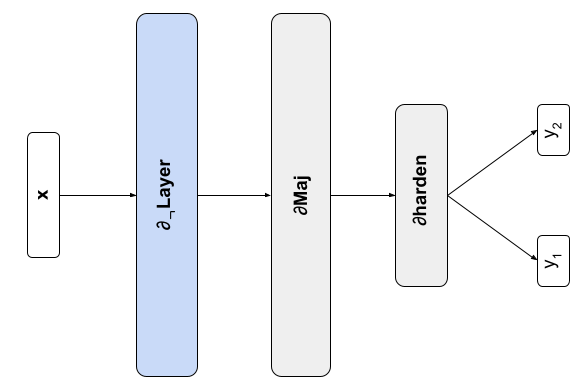
\includegraphics[width=0.49\textwidth]{../toy-example-architecture.png}
	\caption{{\em A $\partial\mathbb{B}$ net to illustrate hardening}. The net concatenates a $\partial_{\neg}\!\operatorname{Layer}$ (of width 8) with a reshaping layer that outputs two vectors, which get reduced, by a $\partial\!\operatorname{Maj}$ operator,  to 2 soft-bits, one for each class label. A final $\partial\!\operatorname{harden}$ layer ensures the loss is a function of hard bits. The net's weights, once hardened, consume $40$ bits ($5$ bytes).}
	\label{fig:toy-example-architecture}
\end{figure}

The $\partial\mathbb{B}$ net specified in Figure \ref{fig:toy-example-architecture} (with 40 soft-bit weights) has two single-bit output ports and is hard-equivalent to the following discrete program (with 40 hard-bit weights):

\begin{lstlisting}[language=Python,style=mystyle,frame=single]
def dbNet(very-cold, cold, warm, very-warm, outside):
return [
ge(sum((sum((sum((sum((sum((sum((sum((sum((sum((sum((sum((sum((sum((sum((sum((sum((sum((sum((sum((sum((0, not(xor(ne(very-cold, 0), w1)))), not(xor(ne(cold, 0), w2)))), not(xor(ne(warm, 0), w3)))), not(xor(ne(very-warm, 0), w4)))), not(xor(ne(outside, 0), w5)))), not(xor(ne(very-cold, 0), w6)))), not(xor(ne(cold, 0), w7)))), not(xor(ne(warm, 0), w8)))), not(xor(ne(very-warm, 0), w9)))), not(xor(ne(outside, 0), w10)))), not(xor(ne(very-cold, 0), w11)))), not(xor(ne(cold, 0), w12)))), not(xor(ne(warm, 0), w13)))), not(xor(ne(very-warm, 0), w14)))), not(xor(ne(outside, 0), w15)))), not(xor(ne(very-cold, 0), w16)))), not(xor(ne(cold, 0), w17)))), not(xor(ne(warm, 0), w18)))), not(xor(ne(very-warm, 0), w19)))), not(xor(ne(outside, 0), w20)))), 11),
ge(sum((sum((sum((sum((sum((sum((sum((sum((sum((sum((sum((sum((sum((sum((sum((sum((sum((sum((sum((sum((0, not(xor(ne(very-cold, 0), w21)))), not(xor(ne(cold, 0), w22)))), not(xor(ne(warm, 0), w23)))), not(xor(ne(very-warm, 0), w24)))), not(xor(ne(outside, 0), w25)))), not(xor(ne(very-cold, 0), w26)))), not(xor(ne(cold, 0), w27)))), not(xor(ne(warm, 0), w28)))), not(xor(ne(very-warm, 0), w29)))), not(xor(ne(outside, 0), w30)))), not(xor(ne(very-cold, 0), w31)))), not(xor(ne(cold, 0), w32)))), not(xor(ne(warm, 0), w33)))), not(xor(ne(very-warm, 0), w34)))), not(xor(ne(outside, 0), w35)))), not(xor(ne(very-cold, 0), w36)))), not(xor(ne(cold, 0), w37)))), not(xor(ne(warm, 0), w38)))), not(xor(ne(very-warm, 0), w39)))), not(xor(ne(outside, 0), w40)))), 11)
]
\end{lstlisting}

\section{Experiments}\label{sec:experiments}

The $\partial\mathbb{B}$ net library is implemented in Flax \cite{flax2020github} and JAX \cite{jax2018github} and available at {\small \url{github.com/Z80coder/db-nets}}. The library supports the specification of a $\partial\mathbb{B}$ net as Python code, which automatically defines (i) the soft-net for training (weights are floats), (ii) a hard-net for inference (weights are booleans), and (iii) a symbolic net for interpretation (weights and inputs are symbols). The symbolic net, when evaluated, interprets its own JAX expression and outputs a description of the discrete program it computes.

We compare the performance of $\partial\mathbb{B}$ nets against standard ML approaches on three problems: the classic Iris dataset, an adversarial noisy XOR problem, and MNIST. 

\subsection{Binary Iris}

\begin{figure}
	\centering
	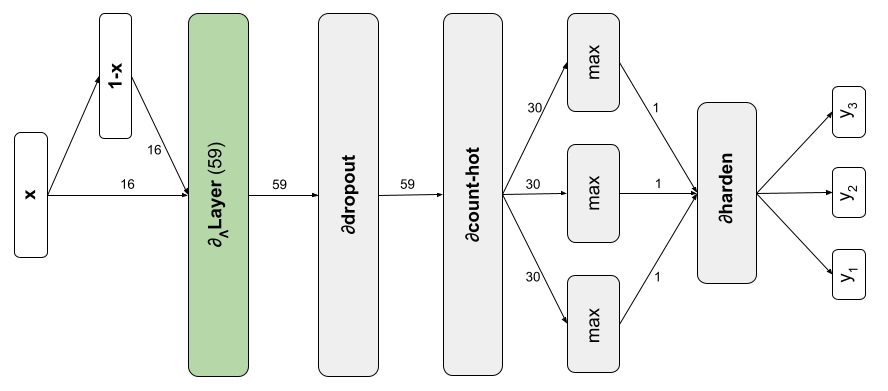
\includegraphics[width=0.75\textwidth]{../binary-iris-architecture.png}
	\caption{{\em A $\partial\mathbb{B}$ net for the binary Iris problem}. The net concatenates the soft-bit input, ${\bf x}$ (length 16), with its negation, ${\bf 1 - x}$, and supplies the resulting vector (length 32) to a $\partial_{\wedge}\!\operatorname{Layer}$ (width 59), a $\partial\!\operatorname{dropout}$ layer for improved generalisation, a $\partial\!\operatorname{count-hot}$ layer that generates a 1-hot vector (width 60) that is reduced by $\operatorname{max}$ to a 1-hot vector of 3 classification bits. A final $\partial\!\operatorname{harden}$ ensures the loss is a function of hard bits. The net's weights, once hardened, consume $236$ bytes.}
	\label{fig:binary-iris-architecture}
\end{figure}


The Iris dataset has 150 examples with 4 inputs (sepal length and width, and petal length and width), and 3 labels ({\em setosa}, {\em versicolour}, and {\em virginica}). We use the binary version of the Iris dataset \cite{binary-iris-dataset} where each input float is represented by 4 bits. We perform 1000 experiments, each with a different random seed. Each experiment randomly partitions the data into 80\% training and 20\% test sets. We initialize the network, described in Figure \ref{fig:binary-iris-architecture}, with all weights $w_{i} = 0.3$ and train for 1000 epochs with the RAdam optimizer and softmax cross-entropy loss. 

We measure the accuracy of the final net to avoid hand-picking the best configuration. Table \ref{tab:binary-iris-results} compares the $\delta\mathbb{B}$ net against other classifiers  \cite{granmo18}. Naive Bayes performs the worst. The Tsetlin machine performs best on this problem, with the $\partial\mathbb{B}$ net second.

\begin{table}[t]
	\centering
	\begin{tabular}{llllll}
		\cline{2-6}
		\multicolumn{1}{c}{}                       & \multicolumn{5}{c}{\textbf{accuracy}}                                                                                                                                                            \\ \cline{2-6} 
		\multicolumn{1}{l|}{}                      & \multicolumn{1}{l|}{mean}                  & \multicolumn{1}{l|}{5 \%ile}       & \multicolumn{1}{l|}{95 \%ile}       & \multicolumn{1}{l|}{min}           & \multicolumn{1}{l|}{max}            \\ \hline
		\multicolumn{1}{|l|}{Tsetlin}              & \multicolumn{1}{l|}{95.0 +/- 0.2}          & \multicolumn{1}{l|}{86.7}          & \multicolumn{1}{l|}{100.0}          & \multicolumn{1}{l|}{80.0}          & \multicolumn{1}{l|}{100.0}          \\ \hline
		\multicolumn{1}{|l|}{$\partial\mathbb{B}$} & \multicolumn{1}{l|}{\textbf{93.9 +/- 0.1}} & \multicolumn{1}{l|}{\textbf{86.7}} & \multicolumn{1}{l|}{\textbf{100.0}} & \multicolumn{1}{l|}{\textbf{80.0}} & \multicolumn{1}{l|}{\textbf{100.0}} \\ \hline
		\multicolumn{1}{|l|}{neural network}       & \multicolumn{1}{l|}{93.8 +/- 0.2}          & \multicolumn{1}{l|}{86.7}          & \multicolumn{1}{l|}{100.0}           & \multicolumn{1}{l|}{80.0}          & \multicolumn{1}{l|}{100.0}           \\ \hline
		\multicolumn{1}{|l|}{SVM}                  & \multicolumn{1}{l|}{93.6 +/- 0.3}          & \multicolumn{1}{l|}{86.7}          & \multicolumn{1}{l|}{100.0}           & \multicolumn{1}{l|}{76.7}          & \multicolumn{1}{l|}{100.0}           \\ \hline
		\multicolumn{1}{|l|}{naive Bayes}          & \multicolumn{1}{l|}{91.6 +/- 0.3}          & \multicolumn{1}{l|}{83.3}          & \multicolumn{1}{l|}{96.7}           & \multicolumn{1}{l|}{70.0}          & \multicolumn{1}{l|}{100.0}           \\ \hline
	\end{tabular}
	\caption{{\em Binary Iris results}  measured over 1000 experiments.}
	\label{tab:binary-iris-results}
\end{table}

\subsection{Noisy XOR}

\begin{figure}
	\centering
	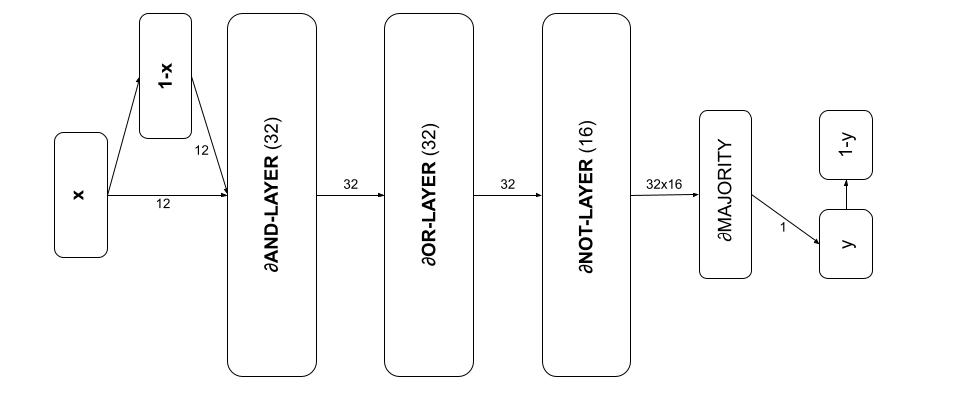
\includegraphics[width=0.75\textwidth]{../noisy-xor-architecture.png}
	\caption{{\em A $\partial\mathbb{B}$ net for the noisy xor problem}. The net concatenates the soft-bit input, ${\bf x}$ (length 12), with its negation, ${\bf 1 - x}$, and supplies the resulting vector (length 24) to a $\partial_{\wedge}\!\!\operatorname{Layer}$ (width 32), $\partial_{\vee}\!\!\operatorname{Layer}$ (width 32),  $\partial_{\neg} \!\operatorname{Layer}$ (width 16), and a final $\partial\!\operatorname{Maj}$ to produce a single soft-bit $y \in [0,1]$ (to predict odd parity) and its negation $1-y$ (to predict even parity). The net's weights, once hardened, consume $288$ bytes.}
	\label{fig:noisy-xor-architecture}
\end{figure}

The noisy XOR dataset \cite{noisy-xor-dataset} is an adversarial parity problem with noisy non-informative features. The dataset consists of 10K examples with 12 boolean inputs and a target label (where 0 = odd and 1 = even) that is a XOR function of 2 of the inputs. The remaining 10 inputs are entirely random. We train on 50\% of the data where, additionally, 40\% of the labels are inverted. We initialize the network described in Figure \ref{fig:noisy-xor-architecture} with random weights distributed close to the hard threshold at $1/2$ (i.e. in the $\partial_{\wedge}\!\operatorname{Layer}$, $w_{i} = 0.501 \times b + 0.3 \times (1-b)$ where $b \sim \operatorname{Bernoulli}(0.01)$; in the $\partial_{\vee}\!\operatorname{Layer}$, $w_{i} = 0.7 \times b + 0.499 \times (1-b)$ where $b \sim \operatorname{Bernoulli}(0.99)$); and in the $\partial_{\neg}\!\operatorname{Layer}$, $w_{i} \sim \operatorname{Uniform}(0.499, 0.501)$. We train for 2000 epochs with the RAdam optimizer and softmax cross-entropy loss. 

We measure the accuracy of the final net on the test data to avoid hand-picking the best configuration. Table \ref{tab:noisy-xor-results} compares the $\partial\mathbb{B}$ net against other classifiers \cite{granmo18}. The high noise causes logistic regression and naive Bayes to randomly guess. The SVM hardly performs better. In contrast, the multilayer neural network, Tsetlin machine, and  $\partial\mathbb{B}$ net all successfully learn the underlying XOR signal. The Tsetlin machine performs best on this problem, with the $\partial\mathbb{B}$ net second.

\begin{table}[t]
	\centering
	\begin{tabular}{llllll}
		\cline{2-6}
		\multicolumn{1}{c}{}                       & \multicolumn{5}{c}{\textbf{accuracy}}                                                                                                                                                            \\ \cline{2-6} 
		\multicolumn{1}{l|}{}                      & \multicolumn{1}{l|}{mean}                  & \multicolumn{1}{l|}{5 \%ile}       & \multicolumn{1}{l|}{95 \%ile}       & \multicolumn{1}{l|}{min}           & \multicolumn{1}{l|}{max}            \\ \hline
		\multicolumn{1}{|l|}{Tsetlin}              & \multicolumn{1}{l|}{99.3 +/- 0.3}          & \multicolumn{1}{l|}{95.9}          & \multicolumn{1}{l|}{100.0}          & \multicolumn{1}{l|}{91.6}          & \multicolumn{1}{l|}{100.0}          \\ \hline
		\multicolumn{1}{|l|}{$\partial\mathbb{B}$} & \multicolumn{1}{l|}{\textbf{97.9 +/- 0.2}} & \multicolumn{1}{l|}{\textbf{95.4}} & \multicolumn{1}{l|}{\textbf{100.0}} & \multicolumn{1}{l|}{\textbf{93.6}} & \multicolumn{1}{l|}{\textbf{100.0}} \\ \hline
		\multicolumn{1}{|l|}{neural network}       & \multicolumn{1}{l|}{95.4 +/- 0.5}          & \multicolumn{1}{l|}{90.1}          & \multicolumn{1}{l|}{98.6}           & \multicolumn{1}{l|}{88.2}          & \multicolumn{1}{l|}{99.9}           \\ \hline
		\multicolumn{1}{|l|}{SVM}                  & \multicolumn{1}{l|}{58.0 +/- 0.3}          & \multicolumn{1}{l|}{56.4}          & \multicolumn{1}{l|}{59.2}           & \multicolumn{1}{l|}{55.4}          & \multicolumn{1}{l|}{66.5}           \\ \hline
		\multicolumn{1}{|l|}{naive Bayes}          & \multicolumn{1}{l|}{49.8 +/- 0.2}          & \multicolumn{1}{l|}{48.3}          & \multicolumn{1}{l|}{51.0}           & \multicolumn{1}{l|}{41.3}          & \multicolumn{1}{l|}{52.7}           \\ \hline
		\multicolumn{1}{|l|}{logistic regression}  & \multicolumn{1}{l|}{49.8 +/- 0.3}          & \multicolumn{1}{l|}{47.8}          & \multicolumn{1}{l|}{51.1}           & \multicolumn{1}{l|}{41.1}          & \multicolumn{1}{l|}{53.1}           \\ \hline
	\end{tabular}
	\caption{{\em Noisy XOR results}  measured over 100 experiments.}
	\label{tab:noisy-xor-results}
\end{table}

\subsection{MNIST}

\begin{figure}
	\centering
	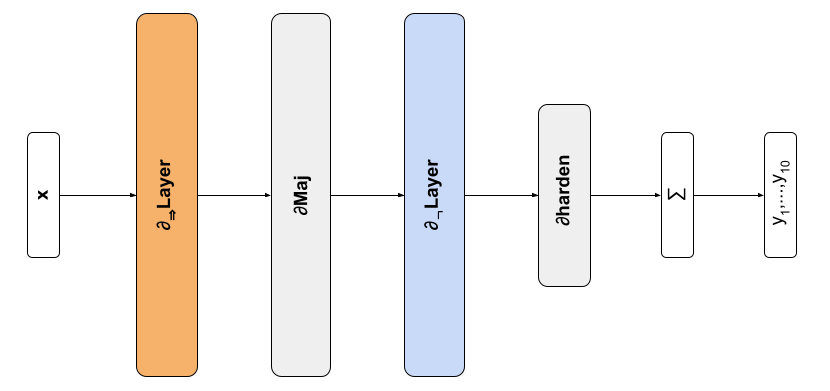
\includegraphics[width=0.75\textwidth]{../mnist-architecture.png}
	\caption{{\em A non-convolutional $\partial\mathbb{B}$ net for MNIST}. The input is a $28\times28$ bit matrix representing an image. The net consists of a $\partial_{\Rightarrow}\!\operatorname{Layer}$ (of width 60, to produce a $2940\times16$ reshaped array), a $\partial\!\operatorname{Maj}$ layer (to produce a vector of size $2940$), a $\partial_{\neg}\!\operatorname{Layer}$ (of width 20, to produce a $20 \times 2940$ array), and a final $\partial\!\operatorname{harden}$ operator to generate hard-bits split into 10 buckets and summed to produce 10 integer logits. The net's weights, once hardened, consume 13.23 kb.}
	\label{fig:mnist-architecture}
\end{figure}


\begin{table}[t]
	\centering
	\begin{tabular}{lc}
		\cline{2-2}
		& \textbf{accuracy}                  \\ \hline
		\multicolumn{1}{|l|}{\em 2-layer NN, 800 HU, cross-entropy loss} & \multicolumn{1}{c|}{98.6} \\ \hline
		\multicolumn{1}{|l|}{Tsetlin}                        & \multicolumn{1}{c|}{98.2 +/- 0.0}  \\ \hline
		\multicolumn{1}{|l|}{\em K-nearest-neighbours, L3}       & \multicolumn{1}{c|}{97.2}          \\ \hline
		\multicolumn{1}{|l|}{$\partial\mathbb{B}$}           & \multicolumn{1}{c|}{\textbf{94.0}} \\ \hline
		\multicolumn{1}{|l|}{Logistic regression}            & \multicolumn{1}{c|}{91.5}          \\ \hline
		\multicolumn{1}{|l|}{\em Linear classifier (1-layer NN)} & \multicolumn{1}{c|}{88.0}          \\ \hline
		\multicolumn{1}{|l|}{Decision tree}                  & \multicolumn{1}{c|}{87.8}          \\ \hline
		\multicolumn{1}{|l|}{Multinomial Naive Bayes}        & \multicolumn{1}{c|}{83.2}          \\ \hline
	\end{tabular}
	\caption{{\em MNIST results}. A classifier in {\em italics} was trained on grey-value pixel data, otherwise the classifier was trained on binarized data. Note: the $\partial\mathbb{B}$ results are from a small model that under-fits the data (due to OOM errors on my GPU). The next draft will include results using a larger $\partial\mathbb{B}$ net.}
	\label{tab:mnist-table}
\end{table}

The MNIST dataset \cite{726791} consists of 60K training and 10K test examples of handwritten digits (0-9). We binarize the data by replacing pixels with grey value greater than 0.3 with 1, otherwise with 0. We initialize the network described in Figure \ref{fig:mnist-architecture} with random weights distributed as $w_{i} = 0.501 \times b + 0.3 \times (1-b)$ where $b \sim \operatorname{Bernoulli}(0.01)$. We train for 1000 epochs with a batch size of 6000 using the RAdam optimizer and softmax cross-entropy loss.

We measure the accuracy on the final net. Table \ref{tab:mnist-table} compares the $\partial\mathbb{B}$ net against other classifiers (reference data taken from \citemyauthoryear{granmo18}). Basic versions of the algorithms (e.g. no convolutional nets) are applied to unenhanced data (e.g. no data augmentation). The aim is to compare raw performance rather than optimise for MNIST. A 2-layer neural network trained on grey-value pixel data performs best. A Tsetlin machine of 40,000 automata each with 256 states (and therefore 40 kb of parameters) trained on binary data achieves $\approx 98.2\%$ accuracy. A $\partial\mathbb{B}$ net with 105,840 soft-bit weights that harden to 1-bit booleans (and therefore 13.23 kb of parameters) trained on binary data achieves $\approx 94.0\%$ accuracy. However, this $\partial\mathbb{B}$ net underfits the training data and we expect better performance from a larger model.

\section{Proofs}

\begin{proposition}\label{prop:not}
	$\partial_{\neg}(x,y) \btright \neg (x \oplus y)$.
	\begin{proof}
		Table \ref{not-table} is the truth table of the boolean function $\neg (x \oplus w)$, where $h(x) = \operatorname{harden}(x)$.
		\begin{table}[h!]
			\begin{center}
				\begin{tabular}{ccccccc}
					\multicolumn{1}{c}{$x$}  &\multicolumn{1}{c}{$y$}  &\multicolumn{1}{c}{$h(x)$}  &\multicolumn{1}{c}{$h(y)$} &\multicolumn{1}{c}{$\partial_{\neg}(x, y)$} &\multicolumn{1}{c}{$h(\partial_{\neg}(x, y))$}
					&\multicolumn{1}{c}{$\neg (h(y) \oplus h(x))$}
					\\ \hline \\
					$\left[0, \frac{1}{2}\right)$ & $\left[0, \frac{1}{2}\right)$ & 0 & 0 & $\left(\frac{1}{2},1\right]$ & 1 & 1\\[0.1cm] 
					$\left(\frac{1}{2}, 1\right]$ & $\left[0, \frac{1}{2}\right)$ &1 & 0 & $\left[0, \frac{1}{2}\right)$ & 0 & 0\\[0.1cm]
					$\left[0, \frac{1}{2}\right)$ & $\left(\frac{1}{2}, 1\right]$ &0 & 1 & $\left[0, \frac{1}{2}\right)$ & 0 & 0\\[0.1cm]
					$\left(\frac{1}{2}, 1\right]$ & $\left(\frac{1}{2}, 1\right]$ &1 & 1 & $\left(\frac{1}{2}, 1\right]$ & 1 & 1\\[0.1cm]
				\end{tabular}
			\end{center}
			\caption{$\partial_{\neg}(x,y) \btright \neg (y \oplus x)$.}\label{not-table}
		\end{table}
	\end{proof}
\end{proposition}

\begin{lemma}\label{prop:augmented}
	If a representative bit, $x_{i}$, is hard-equivalent to a target function, $g$, then so is the augmented bit, $z$.
	\begin{proof}
		As $x_{i}$ is representative then $\operatorname{harden}(x_{i}) = g(\operatorname{harden}({\bf x}))$. The augmented bit, $z$, is given by  \eqref{eq:augmented-bit}:
		\begin{equation*}
		z = \begin{cases}
		1/2 + \bar{\bf x}\times|x_{i} - 1/2| & \text{if } x_{i} > 1/2 \\
		x_{i} + \bar{\bf x}\times|x_{i} - 1/2| & \text{otherwise.}
		\end{cases}
		\end{equation*}
		In consequence,
		\begin{equation*}
		\operatorname{harden}(z) = \begin{cases}
		1 & \text{if } x > 1/2 \\
		0 & \text{otherwise,}
		\end{cases}
		\end{equation*}
		since $x_{i} > 1/2 \Rightarrow z > 1/2$ and $x_{i} \leq 1/2 \Rightarrow z \leq 1/2$. Hence, $\operatorname{harden}(z) = \operatorname{harden}(x_{i}) = g(\operatorname{harden}({\bf x}))$
	\end{proof}
\end{lemma}


\begin{proposition}\label{prop:and}
	$\partial_{\wedge}\!(x,y) \btright x \wedge y$.
	\begin{proof}
		Table \ref{and-table} is the truth table of the boolean function $x \wedge y$, where $h(x) = \operatorname{harden}(x)$..
		\begin{table}[h!]
			\begin{center}
				\begin{tabular}{ccccccc}
					\multicolumn{1}{c}{$x$}  &\multicolumn{1}{c}{$y$}  &\multicolumn{1}{c}{$h(x)$}  &\multicolumn{1}{c}{$h(y)$} &\multicolumn{1}{c}{$\partial_{\wedge}(x, y)$} &\multicolumn{1}{c}{$h(\partial_{\wedge}(x, y))$}
					&\multicolumn{1}{c}{$h(x) \wedge h(y)$}
					\\ \hline \\
					$\left[0, \frac{1}{2}\right)$ & $\left[0, \frac{1}{2}\right)$ & 0 & 0 & $\left[0, \frac{1}{2}\right)$ & 0 & 0\\[0.1cm]
					$\left(\frac{1}{2}, 1\right]$ & $\left[0, \frac{1}{2}\right)$ &1 & 0 & $\left(\frac{1}{4}, \frac{1}{2}\right)$ & 0 & 0\\[0.1cm]
					$\left[0, \frac{1}{2}\right)$ & $\left(\frac{1}{2}, 1\right]$ &0 & 1 & $\left(\frac{1}{4}, \frac{1}{2}\right)$ & 0 & 0\\[0.1cm]
					$\left(\frac{1}{2}, 1\right]$ & $\left(\frac{1}{2}, 1\right]$ &1 & 1 & $\left(\frac{1}{2}, 1\right]$ & 1 & 1\\[0.1cm]
				\end{tabular}
			\end{center}
			\caption{$\partial_{\wedge}(x,y) \btright x \wedge y$.}\label{and-table}
		\end{table}			
	\end{proof}
\end{proposition}

\begin{proposition}\label{prop:or}
	$\partial_{\vee}\!(x,y) \btright x \vee y$.
	\begin{proof}
		Table \ref{or-table} is the truth table of the boolean function $x \vee y$, where $h(x) = \operatorname{harden}(x)$..
		\begin{table}[h!]
			\begin{center}
				\begin{tabular}{ccccccc}
					\multicolumn{1}{c}{$x$}  &\multicolumn{1}{c}{$y$}  &\multicolumn{1}{c}{$h(x)$}  &\multicolumn{1}{c}{$h(y)$} &\multicolumn{1}{c}{$\partial_{\vee}(x, y)$} &\multicolumn{1}{c}{$h(\partial_{\vee}(x, y))$}
					&\multicolumn{1}{c}{$h(x) \vee h(y)$}
					\\ \hline \\
					$\left[0, \frac{1}{2}\right)$ & $\left[0, \frac{1}{2}\right)$ & 0 & 0 & $\left[0,\frac{1}{2}\right)$ & 0 & 0\\[0.1cm]
					$\left(\frac{1}{2}, 1\right]$ & $\left[0, \frac{1}{2}\right)$ &1 & 0 & $\left(\frac{1}{2},1\right]$ & 1 & 1\\[0.1cm]
					$\left[0, \frac{1}{2}\right)$ & $\left(\frac{1}{2}, 1\right]$ &0 & 1 & $\left(\frac{1}{2},1\right]$ & 1 & 1\\[0.1cm]
					$\left(\frac{1}{2}, 1\right]$ & $\left(\frac{1}{2}, 1\right]$ &1 & 1 & $\left(\frac{1}{2},1\right]$ & 1 & 1\\[0.1cm]
				\end{tabular}
			\end{center}
			\caption{$\partial_{\vee}(x,y) \btright x \vee y$.}\label{or-table}
		\end{table}			
	\end{proof}
\end{proposition}

\begin{proposition}\label{prop:implies}
	$\partial_{\Rightarrow}\!(x,y) \btright x \Rightarrow y$.
	\begin{proof}
		Table \ref{implies-table} is the truth table of the boolean function $x \Rightarrow y$, where $h(x) = \operatorname{harden}(x)$..
		\begin{table}[h!]
			\begin{center}
				\begin{tabular}{ccccccc}
					\multicolumn{1}{c}{$x$}  &\multicolumn{1}{c}{$y$}  &\multicolumn{1}{c}{$h(x)$}  &\multicolumn{1}{c}{$h(y)$} &\multicolumn{1}{c}{$\partial_{\Rightarrow}(x, y)$} &\multicolumn{1}{c}{$h(\partial_{\Rightarrow}(x, y))$}
					&\multicolumn{1}{c}{$h(x) \Rightarrow h(y)$}
					\\ \hline \\
					$\left[0, \frac{1}{2}\right)$ & $\left[0, \frac{1}{2}\right)$ & 0 & 0 & $\left(\frac{1}{2}, 1\right]$ & 1 & 0\\[0.1cm]
					$\left(\frac{1}{2}, 1\right]$ & $\left[0, \frac{1}{2}\right)$ &1 & 0 & $\left[0, \frac{1}{2}\right)$ & 0 & 0\\[0.1cm]
					$\left[0, \frac{1}{2}\right)$ & $\left(\frac{1}{2}, 1\right]$ &0 & 1 & $\left(\frac{1}{2},1\right]$ & 1 & 0\\[0.1cm]
					$\left(\frac{1}{2}, 1\right]$ & $\left(\frac{1}{2}, 1\right]$ &1 & 1 & $\left(\frac{1}{2}, \frac{7}{8}\right)$ & 1 & 0\\[0.1cm]
				\end{tabular}
			\end{center}
			\caption{$\partial_{\Rightarrow}(x,y) \btright x \Rightarrow y$.}\label{implies-table}
		\end{table}			
	\end{proof}
\end{proposition}

\begin{lemma}
	\label{lem:maj}
	Let $i$ = $\operatorname{majority-index}({\bf x})$, then the $i$th element of $\operatorname{sort}({\bf x})$ is hard-equivalent to boolean majority, i.e. $\operatorname{harden}(\operatorname{sort}({\bf x})[i]) = \operatorname{Maj}(\operatorname{harden}({\bf x}))$.
	\begin{proof}
		Let $h$ denote the number of bits that are high in ${\bf x} = [x_{1}, \dots, x_{n}]$. Then indices $\{j : n-h+1 \leq j \leq n\}$ are high in $\operatorname{sort}({\bf x})$. If the majority of bits are high, $h \geq \lfloor n/2 + 1 \rfloor$, then index $j=n - \lfloor n/2 + 1 \rfloor + 1 = n - \lfloor n/2 \rfloor = \lceil n/2 \rceil$ is high in $\operatorname{sort}({\bf x})$. $\operatorname{majority-index}$ selects index $i = \lceil n/2 \rceil$ and therefore $i=j$. Hence, if the majority of bits are high then $\operatorname{sort}({\bf x})[i]$ is high. Similarly, if the majority of bits are low, $h < \lfloor n/2 + 1 \rfloor$, then index $j=n - \lfloor n/2 + 1 \rfloor + 1 = n - \lfloor n/2 \rfloor = \lceil n/2 \rceil$ is low in $\operatorname{sort}({\bf x})$. Hence, if the majority of bits are low then $\operatorname{sort}({\bf x})[i]$ is low.
		
		Note that $h \geq \lfloor n/2 + 1 \rfloor$ implies that $\operatorname{Maj}(\operatorname{harden}({\bf x})) \geq \left\lfloor \frac{1}{2} + \frac{1}{n}\left(\frac{n}{2} + 1 - \frac{1}{2} \right) \right\rfloor \geq \left\lfloor 1 + \frac{1}{2n} \right\rfloor = 1$, and $h < \lfloor n/2 + 1 \rfloor$ implies that $\operatorname{Maj}(\operatorname{harden}({\bf x})) < \left\lfloor 1 + \frac{1}{2n} \right\rfloor = 0$.
		
		In consequence, $\operatorname{harden}(\operatorname{sort}({\bf x})[i]) = \operatorname{Maj}(\operatorname{harden}({\bf x}))$ for all $h \in [0,\dots, n]$.
	\end{proof}
\end{lemma}

\begin{theorem}\label{prop:majority}
	$\partial\!\operatorname{Maj} \btright \operatorname{Maj}$.
	\begin{proof}
		$\partial\!\operatorname{Maj}$ augments the representative bit $x_{i} = \operatorname{sort}({\bf x})[\operatorname{majority-index}({\bf x})]$. By lemma \ref{lem:maj} the representative bit is $\btright \operatorname{Maj}(\operatorname{harden}({\bf x}))$.
		By lemma \ref{prop:augmented}, the augmented bit, $\operatorname{augmented-bit}(\operatorname{sort}({\bf x}), \operatorname{majority-index}({\bf x}))$, is also $\btright\!\operatorname{Maj}(\operatorname{harden}({\bf x}))$. Hence $\partial\!\operatorname{Maj} \btright\!\operatorname{Maj}$.
	\end{proof}
\end{theorem}

\begin{proposition}\label{prop:count}
	$\partial\!\operatorname{count-hot} \btright \operatorname{count-hot}$.
	\begin{proof}
		Let $l$ denote the number of bits that are low in ${\bf x} = [x_{1},\dots,x_{n}]$, and let ${\bf y} = \partial\!\operatorname{count-hot}({\bf x})$. Then ${\bf y}[l+1]$ is high and any ${\bf y}[i]$, where $i \neq l+1$, is low. Let ${\bf z} = \operatorname{count-hot}(\operatorname{harden}({\bf x}))$. Then ${\bf z}[l+1]$ is high and any ${\bf z}[i]$, where $i \neq l+1$, is low. Hence, $\operatorname{harden}({\bf y}) = {\bf z}$, and therefore $\partial\!\operatorname{count-hot} \btright \operatorname{count-hot}$.
	\end{proof}
\end{proposition}


\end{document}

\begin{comment}
Define
\begin{equation*}
\begin{aligned}
\partial\text{AND-LAYER}: [0,1]^{n \times m} \times [0,1]^{m} &\to [0,1]^{n}, \\
({\bf W}, {\bf x}) &\mapsto [\partial_{\wedge}\operatorname{Neuron}({\bf W}_{1}, {\bf x}), \dots, \partial_{\wedge}\operatorname{Neuron}({\bf W}_{n}, {\bf x})]
\end{aligned}
\end{equation*}
\end{comment}


\end{document}


% This document was modified from the file originally made available by
% Pat Langley and Andrea Danyluk for ICML-2K. This version was created
% by Iain Murray in 2018, and modified by Alexandre Bouchard in
% 2019 and 2021 and by Csaba Szepesvari, Gang Niu and Sivan Sabato in 2022.
% Modified again in 2023 by Sivan Sabato and Jonathan Scarlett.
% Previous contributors include Dan Roy, Lise Getoor and Tobias
% Scheffer, which was slightly modified from the 2010 version by
% Thorsten Joachims & Johannes Fuernkranz, slightly modified from the
% 2009 version by Kiri Wagstaff and Sam Roweis's 2008 version, which is
% slightly modified from Prasad Tadepalli's 2007 version which is a
% lightly changed version of the previous year's version by Andrew
% Moore, which was in turn edited from those of Kristian Kersting and
% Codrina Lauth. Alex Smola contributed to the algorithmic style files.
